\documentclass[sigconf]{acmart}
\usepackage{amsmath}
\usepackage{graphicx}
\graphicspath{ {./images/} }
\usepackage{caption}
\usepackage{subcaption}
\usepackage[notransparent]{svg}

% Meta information
\title{Image “Outpainting” and Hole Filling: Final Report}
\subtitle{CS 5787 Deep Learning Final Project Report}

\author{Wentao Ye}
\email{wy335@cornell.edu}
\affiliation{%
  \institution{Cornell University}
}

\author{Mitchell Krieger}
\email{mak483@cornell.edu}
\affiliation{%
  \institution{Cornell University}
}

\author{Sebastian Jay}
\email{srj63@cornell.edu}
\affiliation{%
  \institution{Cornell University}
}

% Document begins
\begin{document}

\maketitle

\section*{Team Members}
Wentao Ye (wy335), Mitchell Krieger (mak483), Sebastian Jay (srj63)

\section*{Introduction}
This paper explores the relationship between image inpainting and outpainting by training a model capable of interpolating between two disparate images, blending them seamlessly into a single coherent scene. Inpainting, or image interpolation, is a computer vision task that aims to fill in missing or removed sections of an image, ensuring the completed area integrates smoothly with the existing content. Outpainting, or image extrapolation, generates extensions of an image beyond its original borders.

Drawing inspiration from both inpainting and outpainting, our objective is to generate a transitional region between two images. Traditional inpainting requires an understanding of the context and semantics surrounding the missing area to blend edges seamlessly into the original image. Outpainting, while sharing these challenges, has less context to infer from since it involves extending the image into an unknown space. Additionally, outpainting must handle long-range semantic dependencies, ensuring the generated extensions remain consistent with the original image no matter how far the extrapolation extends. Our task incorporates these challenges and introduces an added complexity: the need for the generated region to be semantically consistent with both images.

\section*{Related Work}
To address the challenges of our task, we leverage deep learning architectures capable of capturing both the semantics at the edges of each image and the relationships between regions across the two images. Historically, Convolutional Neural Networks (CNNs) have been widely used in vision tasks due to their efficiency and ability to learn spatial relationships (LeCun et al., 1998; Krizhevsky et al., 2012). However, CNNs have inherent limitations stemming from their design. Their architecture emphasizes locality, with weight sharing across the entire input, which makes them less adept at capturing long-range dependencies or relationships between non-local regions—a key requirement for complex tasks like ours.

Transformer-based architectures, particularly those employing attention mechanisms, have shown effectiveness in both inpainting and outpainting due to their capacity to model long-range dependencies. For example, Jiahui et al. (2018) demonstrated that incorporating a contextual attention layer significantly improved inpainting performance. Vision Transformers (ViTs) introduced by Dosovitskiy et al. (2020) expanded on this by applying self-attention mechanisms to computer vision tasks, enabling the modeling of global relationships in an image. Further advancements, such as Swin Transformers (Liu et al., 2021), refined the transformer architecture for vision tasks using hierarchical computation and shifted windows to improve efficiency and adaptability. These approaches, however, remain computationally expensive and require large datasets for effective training (d’Ascoli et al., 2021).

Yang et al. (2019) proposed a U-net GAN architecture to perform very long outpainting of a scene in one direction. They used Skip Horizontal Connections to connect each layer of the encoder and decoder in the Unet and an LSTM based Recurrent Transfer Network to transfer the encoded sequences to the decoder. Using this method and generating in multiple steps, they were able to demonstrate long outpainting. Lu et al. (2021) expanded on this work, by combining inpainting, outpainting and image blending to fill in a scene between two images horizontally. They introduced a similar U-net GAN architecture to Yang et al. but also incorporated contextual attention and a Bidirectional Content Transfer module, which used LSTMs as a bottleneck to ensure spatial and semantic consistency across two images. Our work generalizes this approach by extending it to painting between two images in multiple directions.

More recently, diffusion models have gained traction for inpainting and outpainting tasks. Lugmayr et al. (2022) introduced Repaint, which adapted pre-trained denoising diffusion probabilistic models (DDPMs) for inpainting tasks. By modifying the denoising process to condition on known image regions, Repaint successfully handled arbitrary binary masks. Rombach et al. (2022) demonstrated that Stable Diffusion, a diffusion model that operates on the latent space rather than pixel space (Latent Diffusion), achieved state-of-the-art performance in inpainting tasks. Stable Diffusion further enhanced efficiency by conditioning the diffusion process on textual prompts, reducing computational costs while maintaining high performance. However, many of these diffusion models can easily hallucinate, and inpaint or outpaint unknown regions with inauthentic imagery because they are unaware of the true scene. Tang et. al (2024) introduced RealFill which inpaints and outpaints images with results that are conditioned to other images of the original scene, what they refer to as “Authentic Image Completion”. They show that given a set of reference images with different viewpoints, environmental conditions, camera angles, image styles or moved objects they can outpaint a given target image in a way that is accurate to the real scene. To accomplish this, they fine tuned the inpainting stable diffusion model using Correspondence Based Seed Selection, which is a filtering technique that extracts key points in the reference images and scores the generated images by evaluating the correspondence between the references and the target. It then filters and selects the best output based on a threshold.

\section*{Datasets}
We used the \textcolor{red}{\href{https://github.com/z-x-yang/NS-Outpainting}{NS-Outpainting}} dataset to train our models. It is used in the original U-Transformer paper. We also tested our trained model on additional images sourced from the internet.

\section*{Methods}
Architecture
Our approach employs a Generative Adversarial Network (GAN) framework that integrates a U-Net-based generator and a PatchGAN-based discriminator. We chose these architectures to effectively handle the challenges of our interpolation task. Specifically, the generator is responsible for synthesizing the transitional region between two input images, producing outputs that not only blend these images seamlessly but also remain contextually and semantically consistent. The discriminator, on the other hand, aims to distinguish real, fully integrated images from those generated by the model, thereby guiding the generator toward more authentic and coherent results.

Generator (U-Net)
The generator in our framework is inspired by the U-Net architecture, originally proposed by Ronneberger et al. (2015). U-Net is known for its encoder-decoder structure with symmetric skip connections that allow spatial details lost in downsampling operations to be reintroduced at corresponding upsampling stages. This architectural feature is crucial for high-resolution image synthesis tasks, such as ours, because it helps preserve both low-level details (e.g., textures and edges) and high-level semantic cues that are essential for coherent blending.
Our U-Net generator consists of a series of downsampling convolutional layers that progressively capture increasingly abstract features. These encoder stages are followed by a bottleneck layer and a series of corresponding upsampling layers that reconstruct the image back to the original resolution. Skip connections transfer feature maps from the encoder to the decoder, ensuring that spatial and contextual information is retained throughout the synthesis process. The final layer of the generator uses a Tanh activation function to constrain the output pixels to the [-1, 1] range, consistent with our input normalization scheme. This U-Net variant has been successfully applied in tasks like inpainting and outpainting, thus making it a suitable choice for our image interpolation objective.
generator.svg
Discriminator (PatchGAN)
Instead of a standard discriminator that outputs a single scalar probability for the entire image, we adopt a PatchGAN-based discriminator (Isola et al., 2017). The PatchGAN discriminator classifies overlapping local patches of the image as real or fake, rather than the entire image at once. This approach has shown effectiveness in encouraging finer local detail synthesis and prevents the generator from focusing solely on global consistency. By examining smaller regions independently, the PatchGAN discriminator ensures that textures, edges, and local structures are faithfully rendered, ultimately contributing to more realistic intermediate regions.
\begin{figure}[h!]
    \centering
    \includesvg[width=\textwidth]{discriminator}
    \caption{Illustration of the U-Net discriminator architecture.}
    \label{fig:discriminator}
\end{figure}


Training Procedure
\begin{figure}[h!]
    \centering
    \includesvg[width=\textwidth]{generator}
    \caption{Illustration of the U-Net generator architecture.}
    \label{fig:generator}
\end{figure}

Our GAN is trained in an adversarial manner. The generator G takes as input a partially masked image that combines two cropped regions—one from the left-bottom portion of one scene and one from the right-top portion of another scene—thus producing a coherent output that fills in the missing portions. The discriminator D is trained to distinguish the ground-truth combined scene from the generated ones. Throughout training, G aims to produce outputs that are indistinguishable from real images, while D refines its ability to detect generated content, pushing G to create more realistic and semantically consistent results.

Loss Functions
Adversarial Loss:
We employ a standard least-squares GAN objective for the adversarial training (Mao et al., 2017). For the discriminator, the loss compares real and fake patches, encouraging it to assign a high score to real imagery and a low score to generated content. The generator, conversely, seeks to produce patches that the discriminator deems real.
Reconstruction Loss (L1 Loss):
To ensure that the generated content closely matches the ground-truth target image in the masked regions, we use an L1 reconstruction loss:
Structural Similarity (SSIM) Loss:
While pixel-level losses help guide low-level detail, we also incorporate a Structural Similarity Index (SSIM) loss to ensure perceptual quality and to maintain local image structures. The SSIM-based term computes how structurally similar the generated region is to the target, adding a complementary metric that focuses on luminance, contrast, and structural attributes
Perceptual Loss:
Inspired by style transfer and inpainting literature, we include a perceptual loss derived from pre-trained VGG-19 features (Johnson et al., 2016). This loss compares high-level representations of the generated and ground-truth images
Combined Objective
The total generator loss is a weighted combination of these terms:
\[
\mathcal{L}_{G} = \mathcal{L}_{\text{GAN}}(G,D) + \lambda_{\text{recon}}\mathcal{L}_{\text{recon}}(G) + \lambda_{\text{SSIM}}\mathcal{L}_{\text{SSIM}}(G) + \lambda_{\text{perc}}\mathcal{L}_{\text{perc}}(G)
\]

Implementation Details
Our implementation uses PyTorch, and we normalize inputs to the $[-1, 1]$ range. The models are trained using the Adam optimizer (Kingma \& Ba, 2015) with a learning rate of $2 \times 10^{-4}$ and $\beta_1 = 0.5$, $\beta_2 = 0.999$. We periodically save model checkpoints and evaluate intermediate outputs to ensure that the generator’s outputs become progressively more realistic and semantically meaningful.

By combining the strengths of the U-Net generator, PatchGAN discriminator, and multiple complementary loss functions, our method is able to learn complex inter-image relationships and produce visually and contextually coherent transitions between two given images. The following sections detail our experimental setup and results, demonstrating the effectiveness of this approach in bridging visually distinct images into a single, harmonious scene.

\section*{Progress}

\subsection*{1. Reproduction of the paper}
Below is an example of what we were able to achieve within 20 epochs, to fill in an image using the original U-Transformer model. 

\begin{figure}[h]
    \centering
    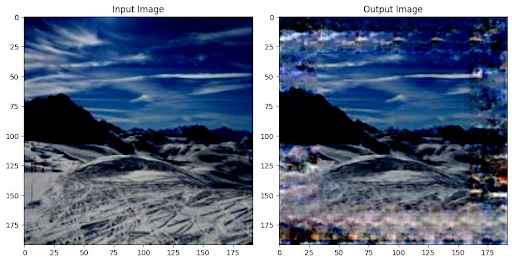
\includegraphics[width=0.8\linewidth]{utransformer.png}
    \caption{Image generated using U-Transformer after 20 epochs.}
\end{figure}

The U-transformer has the following shortcomings:
\begin{itemize}
    \item Fixed size 192
    \item Expensive, requires an NVIDIA A100 GPU in Google Colab to train.
    \item Slow, using an RTX 2070 takes 3 hours per epoch, i.e. 1500 hours for 500 epochs.
    \item Hard code in the Swintransformer model with the center logic so we have to update everything inside the model if we want to crop with different regions.
\end{itemize}

\subsection*{2. New GAN Solution}
The U-Transformer is based on Swin-transformer, which is quite slow, so we want to make it faster and cheaper.

Specifically, we use a GAN framework featuring a \textcolor{red}{\href{https://paperswithcode.com/method/u-net-gan}{U-Net GAN generator}} and a \textcolor{red}{\href{https://paperswithcode.com/method/patchgan}{PatchGAN discriminator}} for image outpainting and scene interpolation. The generator’s encoder-decoder with skip connections creates missing regions, while the discriminator evaluates patch realism. Training optimizes adversarial and reconstruction losses using the Adam optimizer, enabling seamless scene integration. Its benefits are as follows:
\begin{itemize}
    \item Fast, low memory usage, can run on a single RTX 2070
    \item It achieved the results shown below after 20 epochs, training for 3 hours
    \item 256 $\times$ 256 size
    \item \textcolor{red}{\href{https://drive.google.com/file/d/1EORJGbg-rMQ_FNpzz7OSG73Vluro0Lxl/view?usp=sharing}{Weights}}
    \item \textcolor{red}{\href{https://drive.google.com/drive/u/2/folders/1wOD_tgj9k3gUZI9hBL-WtKDS-uvz9m5S}{Code (Google Drive)}}
\end{itemize}

\begin{figure}[h]
    \centering
    \begin{subfigure}[b]{0.3\linewidth}
        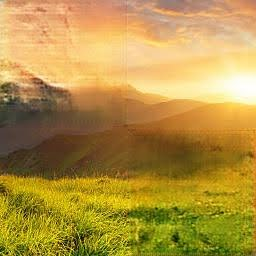
\includegraphics[width=\linewidth]{output1.jpg}
        \caption{Generated}
    \end{subfigure}
    \hfill
    \begin{subfigure}[b]{0.3\linewidth}
        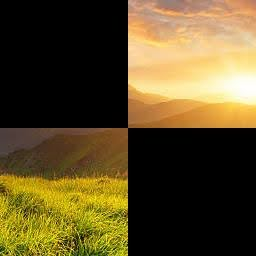
\includegraphics[width=\linewidth]{input1.jpg}
        \caption{Input}
    \end{subfigure}
    \hfill
    \begin{subfigure}[b]{0.3\linewidth}
        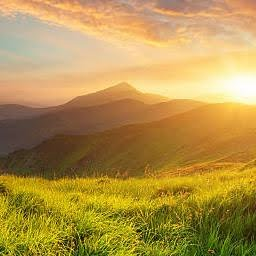
\includegraphics[width=\linewidth]{original1.jpg}
        \caption{Original}
    \end{subfigure}
    \caption{Results from the new GAN model (L-R: Generated, Input, Original).}
\end{figure}

\begin{figure}[h]
    \centering
    \begin{subfigure}[b]{0.3\linewidth}
        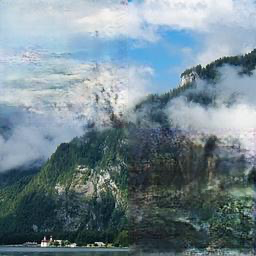
\includegraphics[width=\linewidth]{output2.png}
        \caption{Generated}
    \end{subfigure}
    \hfill
    \begin{subfigure}[b]{0.3\linewidth}
        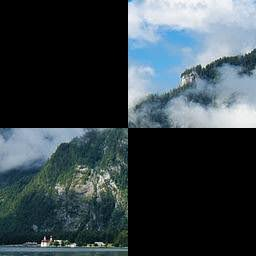
\includegraphics[width=\linewidth]{input2.jpg}
        \caption{Input}
    \end{subfigure}
    \hfill
    \begin{subfigure}[b]{0.3\linewidth}
        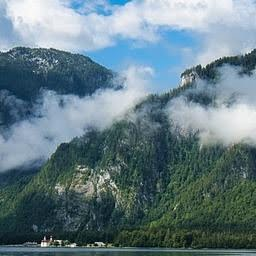
\includegraphics[width=\linewidth]{original2.jpg}
        \caption{Original}
    \end{subfigure}
    \caption{Results from the new GAN model (L-R: Generated, Input, Original).}
\end{figure}

\begin{figure}[h]
    \centering
    \begin{subfigure}[b]{0.3\linewidth}
        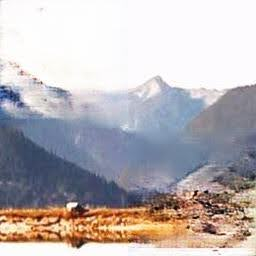
\includegraphics[width=\linewidth]{output3.jpg}
        \caption{Generated}
    \end{subfigure}
    \hfill
    \begin{subfigure}[b]{0.3\linewidth}
        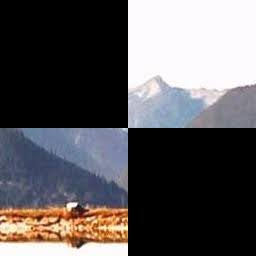
\includegraphics[width=\linewidth]{input3.jpg}
        \caption{Input}
    \end{subfigure}
    \hfill
    \begin{subfigure}[b]{0.3\linewidth}
        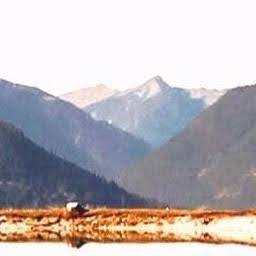
\includegraphics[width=\linewidth]{original3.jpg}
        \caption{Original}
    \end{subfigure}
    \caption{Results from the new GAN model (L-R: Generated, Input, Original).}
\end{figure}

\subsection*{3. New Diffusion Model}
In addition, we looked into additional papers that use diffusion models for tasks like this instead of GANs such as \textcolor{red}{\href{https://arxiv.org/pdf/2201.09865}{“RePaint: Inpainting using Denoising Diffusion Probabilistic Models”}} by Lugmayr et al (2022). Using this research we built an initial diffusion model that inpaints the NS-outpainiting dataset using diffusion. This model was trained on pairs of images and varying masks to represent unknown regions. In the training process, noise is gradually added to only the area where the masks are and MSE is used to attempt to predict this noise over 1000 timesteps. Then the diffusion model attempts to denoise only the pixels that are in the mask. After training for 14 epochs, the diffusion approach shows promising results.  

\begin{itemize}
    \item Trained on NVIDIA A100 in Google Colab, training took ~2.66 hours for 14 epochs
    \item 320 $\times$ 512 Image size
    \item \textcolor{red}{\href{https://drive.google.com/file/d/1-wr7a01nVmRRFrYpwbjaQlc0FIDKINvY/view?usp=sharing}{Weights}}
    \item \textcolor{red}{\href{https://colab.research.google.com/drive/1XZfe98Ox-r8rhJx-8WGiJiJjFm-hb6yO?authuser=2}{Code (Google Drive)}}
\end{itemize}

\begin{figure}[h]
    \centering
    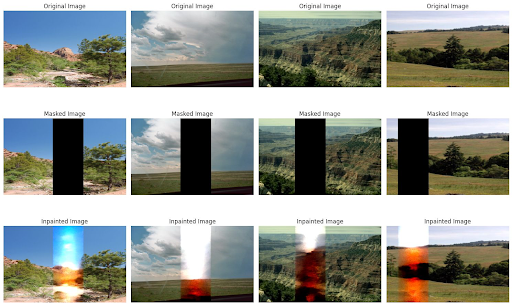
\includegraphics[width=0.8\linewidth]{diffusion_results.png}
    \caption{Original, masked, and inpainted images using diffusion model.}
\end{figure}

\section*{Next Steps}
We would like to train our model on more data, including on images from the RealEstate10K dataset. We’d like to figure out how to make our model predict only the missing parts of the image, rather than regenerating the entire input image including its intact portions.

We will use the following metrics to evaluate our results:
\begin{itemize}
    \item \textbf{FID (Frechet Inception Distance)}: Assesses the similarity between the distributions of generated and real images, measuring both quality and diversity.
    \item \textbf{PSNR (Peak Signal-to-Noise Ratio)}: Evaluates the reconstruction quality by quantifying the pixel-level differences between generated and original images.
    \item \textbf{SSIM (Structural Similarity Index)}: Measures the structural similarity and perceptual quality between generated and ground truth images.
    \item \textbf{IS (Inception Score)}: Evaluates the clarity and diversity of generated images using a pre-trained Inception model.
\end{itemize}

\subsection*{Additional TODOs for GAN:}
\begin{itemize}
    \item Randomize location and size of cropped areas in training images (hard based on GAN)
    \item Bigger image size
    \item Smaller crop size
    \item Generate only the missing part, instead of using mask (hard based on GAN)
    \item Use two different images as each input sample
    \item Update loss function to optimize the performance
\end{itemize}

\subsection*{Additional TODOs for Diffusion:}
\begin{itemize}
    \item Train for additional epochs
    \item More masks of varying shapes
    \item Use Wasserstein Loss to better anchor generated inpaints to the original image, and penalize excess RGB color divergence in output image from input
    \item Better tune Gaussian Blur to make the boundary between the inpaint and the original model less stark.
\end{itemize}

\end{document}
